\BourbakiExercises{习题}

\begin{enumerate}
\def\labelenumi{\arabic{enumi})}
\tightlist
\item
  设 G 是一个群，Z{[}G{]} 是 G 在 Z 上的代数；我们把 G 与 Z{[}G{]} 的典范基等同起来。设 M 是一个 Z{[}G{]}-模，也就是说，一个赋予 G 的作用（保持其群结构的）的交换群。对任何整数 \(n \geqslant 0\)，用 \(C^{n}(G, M)\) 表示从 \(G^{n}\) 到 M 的映射所成的群；令 \(C^{n}(G, M) = 0\)（对 n \textless{} 0）。用下面的公式定义一个同态 \(d^{n}: C^{n}(G, M) \to C^{n+1}(G, M)\)：
\end{enumerate}

\[
\begin{array}{c} (d ^ {n} c) (g _ {0}, \ldots , g _ {n}) = g _ {0}   c (g _ {1}, \ldots , g _ {n}) + \sum_ {i = 0} ^ {n - 1} (- 1) ^ {i + 1} c (g _ {0}, \ldots , g _ {i} g _ {i + 1}, \ldots , g _ {n}) \\ \qquad \qquad \qquad \qquad \qquad \qquad \qquad \qquad \qquad \qquad \qquad \qquad + (- 1) ^ {n + 1} c (g _ {0}, \ldots , g _ {n - 1})  . \end{array}
\]

对任何整数 \(n\)，令 \(Z^n(\mathrm{G},\mathrm{M}) = \operatorname{Ker} d^n\) 与 \(B^n(\mathrm{G},\mathrm{M}) = \operatorname{Im} d^n\)。

\begin{enumerate}
\def\labelenumi{\alph{enumi})}
\tightlist
\item
  证明 \(\mathrm{B}^n (\mathrm{G},\mathrm{M})\) 包含于 \(\mathbf{Z}^n (\mathbf{G},\mathbf{M})\)。
\end{enumerate}

令 \(\mathrm{H}^{n}(\mathrm{G},\mathrm{M})=\mathrm{Z}^{n}(\mathrm{G},\mathrm{M})/\mathrm{B}^{n}(\mathrm{G},\mathrm{M})\)。群 \(\mathrm{H}^{0}(\mathrm{G},\mathrm{M})\) 是 M 中被 G 的作用固定的元素所成之集。群 \(\mathrm{Z}^{1}(\mathrm{G},\mathrm{M})\) 是映射 \(f:\mathrm{G}\to\mathrm{M}\) 所成的群，其中 f 满足 \(f(gg')=f(g)+gf(g')\)，而 \(\mathrm{B}^{1}(\mathrm{G},\mathrm{M})\) 是如下映射 f 所成的子群：存在 \(m\in M\) 使得 \(f(g)=gm-m\)（参看 I, §6, 第 148 页，习题 7）。

\begin{enumerate}
\def\labelenumi{\alph{enumi})}
\setcounter{enumi}{1}
\item
  设 N 是一个 Z{[}G{]}-模，并设 \(u : M \to N\) 是一个 Z{[}G{]}-线性映射。对每个整数 n，映射 \(c \mapsto u \circ c\) 是从 \(C^{n}(G, M)\) 到 \(C^{n}(G, N)\) 的同态，它把 \(Z^{n}(G, M)\) 映入 \(Z^{n}(G, N)\)，把 \(B^{n}(G, M)\) 映入 \(B^{n}(G, N)\)，从而诱导一个从 \(H^{n}(G, M)\) 到 \(H^{n}(G, N)\) 的同态，我们把它记作 \(H^{n}(G, u)\) 或简记作 \(H^{n}(u)\)。若 \(v : N \to P\) 是 Z{[}G{]}-模的一个同态，则我们有 \(H^{n}(v \circ u) = H^{n}(v) \circ H^{n}(u)\)。
\item
  设 \(0 \to M' \xrightarrow{\iota} M \xrightarrow{\pi} M'' \to 0\) 是 Z{[}G{]}-模的一个正合列。设 n 是一个整数，并设 \(x''\) 是 \(\mathrm{H}^{n}(\mathrm{G},\mathrm{M}'')\) 的一个元素，即元素 \(c'' \in Z^{n}(\mathrm{G},\mathrm{M}'')\) 的类。设 \(c \in \mathrm{C}^{n}(\mathrm{G},\mathrm{M})\) 满足 \(\pi \circ c = c''\)。证明存在一个元素 \(c' \in \mathrm{Z}^{n+1}(\mathrm{G},\mathrm{M}')\) 使得 \(\iota \circ c' = d^{n}(c)\)，并且 \(c'\) 在 \(\mathrm{H}^{n+1}(\mathrm{G},\mathrm{M}')\) 中的类只依赖于 \(x''\)；我们把该类记作 \(\partial^{n}(x'')\)。映射 \(\partial^{n}: \mathrm{H}^{n}(\mathrm{G},\mathrm{M}'') \to \mathrm{H}^{n+1}(\mathrm{G},\mathrm{M}')\) 是一个同态（“连接同态”）。证明序列
\end{enumerate}

\[
\dots \longrightarrow \mathrm{H} ^ {n} (\mathrm{G}, \mathrm{M} ^ {\prime}) \stackrel {{\mathrm{H} ^ {n} (\iota)}} {{\longrightarrow}} \mathrm{H} ^ {n} (\mathrm{G}, \mathrm{M}) \stackrel {{\mathrm{H} ^ {n} (\pi)}} {{\longrightarrow}} \mathrm{H} ^ {n} (\mathrm{G}, \mathrm{M} ^ {\prime \prime}) \stackrel {{\partial^ {n}}} {{\longrightarrow}} \mathrm{H} ^ {n + 1} (\mathrm{G}, \mathrm{M} ^ {\prime}) \longrightarrow \dots
\]

是正合的。

\begin{enumerate}
\def\labelenumi{\arabic{enumi})}
\setcounter{enumi}{1}
\tightlist
\item
  设 \(\varphi : \mathrm{H} \to \mathrm{G}\) 是一个群同态，M 是一个 Z{[}G{]}-模，N 是一个 Z{[}H{]}-模，并设 \(u : \mathrm{M} \to \mathrm{N}\) 是交换群的一个同态。我们说 \(\varphi\) 与 \(u\) 是相容的，如果我们有 \(u(\varphi(h)x) = hu(x)\)（对每个 \(h \in \mathrm{H}\) 与每个 \(x \in \mathrm{M}\)）。
\end{enumerate}

\begin{enumerate}
\def\labelenumi{\alph{enumi})}
\item
  对 \(n \geqslant 0\)，设 \(\varphi^{n}: H^{n} \to G^{n}\) 是由 \(\varphi\) 诱导的映射；若 \(\varphi\) 与 u 相容，则同态 \(c \mapsto u \circ c \circ \varphi^{n}\)（从 \(C^{n}(G, M)\) 到 \(C^{n}(H, N)\) 的）把 \(Z^{n}(G, M)\) 映入 \(Z^{n}(H, N)\)，把 \(B^{n}(G, M)\) 映入 \(B^{n}(H, N)\)，从而诱导一个同态 \(H^{n}(\varphi, u)\)（从 \(H^{n}(G, M)\) 到 \(H^{n}(H, N)\) 的）。
\item
  设 \(\psi : \mathrm{K} \to \mathrm{H}\) 是另一个群同态，P 是一个 Z{[}K{]}-模，并设 \(v: \mathrm{N} \to \mathrm{P}\) 是交换群的一个同态。若 \(\varphi\) 与 \(u\) 相容，且 \(\psi\) 与 \(v\) 也相容，则我们有 \(\mathrm{H}^n(\varphi \circ \psi, v \circ u) = \mathrm{H}^n(\psi, v) \circ \mathrm{H}^n(\varphi, u)\)。
\item
  考虑一个交换图
\end{enumerate}

\pandocbounded{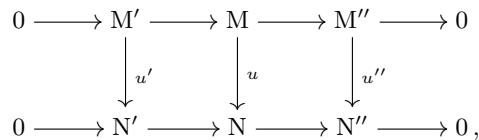
\includegraphics[keepaspectratio]{images/part002_92bb4337.jpg}}

其中第一行（相应地，第二行）是 Z{[}G{]}-模（相应地，Z{[}H{]}-模）的一个正合列，且 \(u', u, u''\) 与 \(\varphi\) 相容。证明图

\[
\begin{array}{l} \dots \longrightarrow \mathrm{H} ^ {n} (\mathrm{G}, \mathrm{M} ^ {\prime}) \longrightarrow \mathrm{H} ^ {n} (\mathrm{G}, \mathrm{M}) \longrightarrow \mathrm{H} ^ {n} (\mathrm{G}, \mathrm{M} ^ {\prime \prime}) \longrightarrow \mathrm{H} ^ {n + 1} (\mathrm{G}, \mathrm{M} ^ {\prime}) \longrightarrow \dots \\ \Biggl \downarrow_ {\mathrm{H} ^ {n} (\varphi , u ^ {\prime})} \qquad \Biggl \downarrow_ {\mathrm{H} ^ {n} (\varphi , u)} \qquad \Biggl \downarrow_ {\mathrm{H} ^ {n} (\varphi , u ^ {\prime \prime})} \qquad \Biggl \downarrow_ {\mathrm{H} ^ {n + 1} (\varphi , u)} \\ \dots \longrightarrow \mathrm{H} ^ {n} (\mathrm{H}, \mathrm{N} ^ {\prime}) \longrightarrow \mathrm{H} ^ {n} (\mathrm{H}, \mathrm{N}) \longrightarrow \mathrm{H} ^ {n} (\mathrm{H}, \mathrm{N} ^ {\prime \prime}) \longrightarrow \mathrm{H} ^ {n + 1} (\mathrm{H}, \mathrm{N} ^ {\prime}) \longrightarrow \dots \end{array}
\]

（其水平各行是习题 1, c) 中定义的长正合列）是交换的。

\begin{enumerate}
\def\labelenumi{\alph{enumi})}
\setcounter{enumi}{3}
\item
  例：若 H = G，则映射 u 与 \(Id_{G}\) 相容当且仅当它是 Z{[}G{]}-线性的，且我们有 \(\mathrm{H}^{n}(\mathrm{Id}_{\mathrm{G}}, u) = \mathrm{H}^{n}(\mathrm{G}, u)\)。若 N 等于 M（赋予一个 Z{[}G{]}-模结构，即由 \(\varphi\) 诱导的那一个），则同态 \(\varphi\) 与 \(1_{M}\) 相容；我们用 \(\operatorname{Res}^{q} : \mathrm{H}^{q}(\mathrm{G}, \mathrm{M}) \to \mathrm{H}^{q}(\mathrm{H}, \mathrm{M})\) 表示同态 \(\mathrm{H}^{q}(\varphi, 1_{\mathrm{M}})\)（“限制同态”）。
\item
  设 H 是 G 的一个正规子群，并设 \(M^{H}\) 是 M 中在 H 下不变的元素所成的子群（赋予由 G 的作用通过取商而诱导的 G/H 的作用）。典范满射 \(p: G \rightarrow G/H\) 与典范单射 \(j: M^{H} \rightarrow M\) 是相容的；我们用 \(\operatorname{Inf}^{q}: \operatorname{H}^{q}(\operatorname{G}/\operatorname{H}, \operatorname{M}^{\operatorname{H}}) \to \operatorname{H}^{q}(\operatorname{G}, \operatorname{M})\) 表示同态 \(\operatorname{H}^{q}(p, j)\)（“膨胀同态”）。证明序列
\end{enumerate}

\[
0 \to \mathrm{H} ^ {1} (\mathrm{G} / \mathrm{H}, \mathrm{M} ^ {\mathrm{H}}) \xrightarrow {\operatorname{Inf} ^ {1}} \mathrm{H} ^ {1} (\mathrm{G}, \mathrm{M}) \xrightarrow {\operatorname{Res} ^ {1}} \mathrm{H} ^ {1} (\mathrm{H}, \mathrm{M})
\]

是正合的。此外，若 \(\mathrm{H}^1 (\mathrm{H},\mathrm{M})\) 为零，则序列

\[
0 \to \mathrm{H} ^ {2} (\mathrm{G} / \mathrm{H}, \mathrm{M} ^ {\mathrm{H}}) \xrightarrow {\operatorname{Inf} ^ {2}} \mathrm{H} ^ {2} (\mathrm{G}, \mathrm{M}) \xrightarrow {\operatorname{Res} ^ {2}} \mathrm{H} ^ {2} (\mathrm{H}, \mathrm{M})
\]

是正合的。

¶ 3) 设 G 是一个群，M 是一个 Z{[}G{]}-模。让 G 作用在 C \(^{1}\) (G,M) 上，其作法是把 \((g,f)\in\mathrm{G}\times\mathrm{C}^{1}(\mathrm{G},\mathrm{M})\) 映为 G 上的函数 \(h\mapsto gf(g^{-1}h)\)。回顾（I, §6, 第 149 页，习题 8），M 上的一个 G-平均是一个 Z{[}G{]}-线性映射 \(\mu:C^{1}(\mathrm{G},\mathrm{M})\to\mathrm{M}\)，它满足 \(\mu(c_{x})=x\)，其中 \(c_{x}\) 表示取值 \(x\in\mathrm{M}\) 的常值函数。

\begin{enumerate}
\def\labelenumi{\alph{enumi})}
\item
  证明若 M 容许一个 G-平均，则 \(\mathrm{H}^{n}(\mathrm{G},\mathrm{M})\) 为零（对 \(n \geqslant 1\)）。（对 \(q \geqslant 1\)，设 \(h^{q}: \mathrm{C}^{q}(\mathrm{G},\mathrm{M}) \to \mathrm{C}^{q-1}(\mathrm{G},\mathrm{M})\) 是如下同态：对 G 中的 \(g_{1}, \ldots, g_{q-1}\) 与 \(c \in \mathrm{C}^{q}(\mathrm{G}, \mathrm{M})\)，把 \(h^{q}(c)(g_{1}, \ldots, g_{q-1})\) 定义为 \(\mu\) 作用于函数 \(g \mapsto c(g_{1}, \ldots, g_{q-1}, (g_{1} \cdots g_{q-1})^{-1}g)\) 所得的像。证明等式 \(h^{q+1} \circ d^{q} + d^{q-1} \circ h^{q} = 1_{\mathrm{C}^{q}(\mathrm{G}, \mathrm{M})}\)。
\item
  设 A 是一个交换群；用 \(\mathcal{F}(\mathrm{G},\mathrm{A})\) 表示从 G 到 A 的映射所成的群（赋予由 \({}^{g}f(h)=f(hg)\)（对 G 中的 g, h 与 \(\mathcal{F}(\mathrm{G},\mathrm{A})\) 中的 f）定义的 G 的作用）。对从 G 到 \(\mathcal{F}(\mathrm{G},\mathrm{A})\) 的任何映射 c，用 \(\mu(c)\) 表示从 G 到 A 的映射 \(g\mapsto c(g^{-1})(g)\)。证明 \(\mu\) 是 \(\mathcal{F}(\mathrm{G},\mathrm{A})\) 上的一个 G-平均；因此我们有 \(\mathrm{H}^{q}(\mathrm{G},\mathcal{F}(\mathrm{G},\mathrm{A}))=0\)（对 \(q\geqslant1\)）。
\item
  设 \(j: M \to \mathcal{F}(G, M)\) 是把 M 的元素 m 映为函数 \(g \mapsto gm\) 的映射，并设 \(M'\) 是它的余核。证明 j 是单射且是 Z{[}G{]}-线性的。由此推出同态 \(\partial^{q}: H^{q}(G, M') \to H^{q+1}(G, M)\) 是双射（对 \(q \geqslant 1\)）。
\item
  设 L 是交换域 K 的一个有限伽罗瓦扩张，并设 G 是它的伽罗瓦群。由 b) 与正规基定理（V, §10, No.~9, 第 73 页）推出，群 \(\mathrm{H}^{n}(\mathrm{G},\mathrm{L})\) 为零（对 \(n \geqslant 1\)）。
\end{enumerate}

¶ 4) 设 G 是一个群，H 是 G 的一个子群。对任何 Z{[}H{]}-模 N，用 \(\widetilde{N}\) 表示群 \(\operatorname{Hom}_{\mathbf{Z}[H]}(\mathbf{Z}[G], N)\)（赋予由 Z{[}G{]} 上的右 Z{[}G{]}-模结构诱导的一个 Z{[}G{]}-模结构）。

\begin{enumerate}
\def\labelenumi{\alph{enumi})}
\item
  证明 \(\widetilde{\mathbf{N}}\) 可与一个 \(\mathbf{Z}[\mathrm{G}]\)-子模等同起来，即 \(\mathcal{F}(\mathrm{G},\mathrm{N})\)（习题 3）中由映射 \(f\) 所组成的、满足 \(f(hg) = hf(g)\)（对每个 \(h\in \mathrm{H}\) 与每个 \(g\in \mathrm{G}\)）的那个子模。若 \(\mathrm{A}\) 是一个交换群，则 \(\mathbf{Z}[\mathrm{G}]\)-模 \(\widetilde{\mathcal{F}(\mathrm{H},\mathrm{A})}\) 典范同构于 \(\mathcal{F}(\mathrm{G},\mathrm{A})\)。
\item
  设 \(0 \rightarrow N' \stackrel{i}{\rightarrow} N \stackrel{p}{\rightarrow} N'' \rightarrow 0\) 是 Z{[}H{]}-模的一个正合列；序列
\end{enumerate}

\[
0 \longrightarrow \widetilde {\mathrm{N}} ^ {\prime} \xrightarrow {\operatorname{Hom} (1 , i)} \widetilde {\mathrm{N}} \xrightarrow {\operatorname{Hom} (1 , p)} \widetilde {\mathrm{N}} ^ {\prime \prime} \longrightarrow 0
\]

是正合的（注意 \(\mathbf{Z}[\mathrm{H}]\)-模 \(\mathbf{Z}[\mathrm{G}]\) 是自由的）。

\begin{enumerate}
\def\labelenumi{\alph{enumi})}
\setcounter{enumi}{2}
\tightlist
\item
  设 \(u_{N} : \widetilde{N} \to N\) 是映射 \(f \mapsto f(1)\)；它与典范单射 \(i : H \to G\) 相容（习题 2）。证明同态
\end{enumerate}

\[
\mathrm{H} ^ {q} (i, u _ {\mathrm{N}}): \mathrm{H} ^ {q} (\mathrm{G}, \widetilde {\mathrm{N}}) \to \mathrm{H} ^ {q} (\mathrm{H}, \mathrm{N})
\]

对每个 \(q \geqslant 0\) 是双射（先处理 q = 0 的情形，然后利用上述结果、习题 3, c) 以及习题 2, c)，对 q 作归纳法推理）。

\begin{enumerate}
\def\labelenumi{\alph{enumi})}
\setcounter{enumi}{3}
\item
  假设 H 在 G 中有有限指标 n。设 M 是一个 Z{[}G{]}-模，我们通过限制标量把它看作一个 Z{[}H{]}-模。设 \(f \in \widetilde{M}\)；元素 \(g^{-1}f(g)\) 只依赖于 g 的右陪集 Hg。令 \(\pi(f) = \sum_{Hg \in H \setminus G} g^{-1}f(g)\)。证明 \(\pi\) 是一个 Z{[}G{]}-线性同态（从 \(\widetilde{M}\) 到 M 的）。对任何整数 \(q \geqslant 0\)，用 \(\operatorname{Cor}^{q}: \mathrm{H}^{q}(\mathrm{H}, \mathrm{M}) \to \mathrm{H}^{q}(\mathrm{G}, \mathrm{M})\) 表示同态 \(\mathrm{H}^{q}(\pi) \circ \mathrm{H}^{q}(i, u_{\mathrm{M}})^{-1}\)（“余限制同态”）。
\item
  证明自同态 \(Cor^{q} \circ Res^{q}\)（\(H^{q}(G, M)\) 的）是乘以 n 的映射（先处理 q = 0 的情形，然后按 c) 的证明中的做法处理一般情形）。
\item
  假设 G 是有限的；证明对每个 Z{[}G{]}-模 M 与每个整数 \(q \geqslant 1\)，群 \(\mathrm{H}^{q}(\mathrm{G}, \mathrm{M})\) 被 G 的阶零化。
\end{enumerate}

\begin{enumerate}
\def\labelenumi{\arabic{enumi})}
\setcounter{enumi}{4}
\tightlist
\item
  设 G 是一个群，M 是一个不一定交换的群（赋予一个同态 \(\varphi: G \to \text{Aut}(M)\)）；对 \(g \in G\) 与 \(m \in M\)，令 \(^{g}m = \varphi(g)(m)\)。用 \(H^{0}(G, M)\) 表示 M 中被 G 的作用固定的元素所成的子群；它的单位元素称为 \(H^{0}(G, M)\) 的标记元素或特异元素。设 \(Z^{1}(G, M)\) 是映射 \(c: G \to M\) 所成之集，其中 c 满足 \(c(gh) = c(g)^{g}c(h)\)（对 G 中的 g, h）。对 \(c \in Z^{1}(G, M)\) 与 \(m \in M\)，映射 \(g \mapsto mc(g)(^g m)^{-1}\) 属于 \(Z^{1}(G, M)\)；这就定义了群 M 在 \(Z^{1}(G, M)\) 上的一个作用。商集记作 \(H^{1}(G, M)\)；它带有一个标记元素，即取值 1 的常值映射的类。若 M 是交换的，则集合 \(H^{1}(G, M)\) 与习题 1 中定义的那个重合。
\end{enumerate}

\begin{enumerate}
\def\labelenumi{\alph{enumi})}
\item
  设 N 是另一个赋予 G 的作用的群，并设 \(u: M \to N\) 是一个与 G 的作用相容的群同态。对 i = 0, 1，定义同态 \(\mathrm{H}^{i}(u): \mathrm{H}^{i}(\mathrm{G}, \mathrm{M}) \to \mathrm{H}^{i}(\mathrm{G}, \mathrm{N})\)，它们把 \(\mathrm{H}^{i}(\mathrm{G}, \mathrm{M})\) 的标记元素映为 \(\mathrm{H}^{i}(\mathrm{G}, \mathrm{N})\) 的标记元素。
\item
  设 \(0 \to M' \xrightarrow{\iota} M \xrightarrow{\pi} M'' \to 0\) 是带 G 中算子的群的一个正合列。设 \(x'' \in \mathrm{H}^0(\mathrm{G}, \mathrm{M}'')\)，并设 x 是 M 的一个元素，使得 \(\pi(x) = x''\)。证明存在一个元素 \(c' \in \mathrm{Z}^1(\mathrm{G}, \mathrm{M}')\)，使得 \(\iota \circ c'(g) = g^{-1}c(g)\)（对每个 \(g \in G\)），并且 \(c'\) 在 \(\mathrm{H}^1(\mathrm{G}, \mathrm{M}')\) 中的类只依赖于 \(x''\)；我们把该类记作 \(\partial(x'')\)。证明序列
\end{enumerate}

\[
0 \to \mathrm{H} ^ {0} (\mathrm{G}, \mathrm{M} ^ {\prime}) \xrightarrow {\mathrm{H} ^ {0} (\iota)} \mathrm{H} ^ {0} (\mathrm{G}, \mathrm{M}) \xrightarrow {\mathrm{H} ^ {0} (\pi)} \mathrm{H} ^ {0} (\mathrm{G}, \mathrm{M} ^ {\prime \prime}) \xrightarrow {\partial}
\]

\[
\mathrm{H} ^ {1} (\mathrm{G}, \mathrm{M} ^ {\prime}) \xrightarrow {\mathrm{H} ^ {1} (\iota)} \mathrm{H} ^ {1} (\mathrm{G}, \mathrm{M}) \xrightarrow {\mathrm{H} ^ {1} (\pi)} \mathrm{H} ^ {1} (\mathrm{G}, \mathrm{M} ^ {\prime \prime})
\]

是正合的（映射序列 \(G \xrightarrow{i} F \xrightarrow{p} E\)（其中集合 E 带有一个标记元素 e）称为在 F 处正合，如果 \(\operatorname{Im}(i) = p^{-1}(e)\)）。

\begin{enumerate}
\def\labelenumi{\alph{enumi})}
\setcounter{enumi}{2}
\item
  此外，假设 \(M'\) 包含在 M 的中心内。构造一个映射 \(\partial^{1}: H^{1}(G, M'') \to H^{2}(G, M')\)，使得单位元素在 \(\partial^{1}\) 下的逆像是 \(H^{1}(\pi)\) 的像。再定义群 \(H^{1}(G, M')\) 在集合 \(H^{1}(G, M)\) 上的一个作用，使得两个元素在这个作用下共轭当且仅当它们在 \(H^{1}(\pi)\) 下有相同的像。
\item
  设 K 是一个交换域，L 是 K 的一个有限伽罗瓦扩张（伽罗瓦群为 G），n 是一个整数。让 G 作用在群 \(\mathbf{GL}_{n}(\mathrm{L})\) 上，其作法是令 \(\sigma A = (\sigma(a_{ij}))\)（对 \(\sigma \in G\) 与 \(A = (a_{ij}) \in \mathbf{GL}_{n}(\mathrm{L})\)）。由 V, §10, No.~5, 第 64 页，命题 9 推出，集合 \(\mathrm{H}^{1}(\mathrm{G}, \mathbf{GL}_{n}(\mathrm{L}))\) 只含一个元素（“希尔伯特定理 90”）。
\end{enumerate}

¶ 6) 设 L 是交换域 K 的一个有限伽罗瓦扩张（伽罗瓦群为 G）。设 V 与 V' 是 K-向量空间，w（相应地，w'）是 V（相应地，V'）上一个 \((p,q)\) 型张量。从 \((V,w)\) 到 \((V',w')\) 的一个 L-同构是一个 L-线性同构 \(u:V_{(L)}\to V_{(L)}'\)，使得 \(u^{\otimes p}\otimes(^{t}u^{-1})^{\otimes q}\) 把 w 的像映为 \(w'\) 的像。我们用 \(\operatorname{Aut}_{\mathrm{L}}(\mathrm{V},w)\) 表示 \((\mathrm{V},w)\) 的 L-自同构所成的群，G 在其上通过 \(\sigma\varphi=(1_{\mathrm{V}}\otimes\sigma)\circ\varphi\circ(1_{\mathrm{V}}\otimes\sigma)^{-1}\) 作用。

\begin{enumerate}
\def\labelenumi{\alph{enumi})}
\item
  设 u 是从 \((\mathrm{V}, w)\) 到 \((\mathrm{V}^{\prime}, w^{\prime})\) 的一个 L-同构，\(\sigma\) 是 G 的一个元素；映射 \(\sigma u = (1_{\mathrm{V}^{\prime}} \otimes \sigma) \circ u \circ (1_{\mathrm{V}} \otimes \sigma)^{-1}\) 是从 \((\mathrm{V}, w)\) 到 \((\mathrm{V}^{\prime}, w^{\prime})\) 的一个 L-同构，从而 \(c(\sigma) = u^{-1} \circ \sigma u\) 是 \(\operatorname{Aut}_{\mathrm{L}}(\mathrm{V}, w)\) 的一个元素。证明映射 \(c : G \to \operatorname{Aut}_{\mathrm{L}}(\mathrm{V}, w)\) 属于 \(Z^{1}(\mathrm{G}, \operatorname{Aut}_{\mathrm{L}}(\mathrm{V}, w))\)，并且它的类 \(\theta(\mathrm{V}^{\prime}, w^{\prime})\)（在 \(H^{1}(\mathrm{G}, \operatorname{Aut}_{\mathrm{L}}(\mathrm{V}, w))\) 中的）不依赖于 u 的选取。
\item
  证明映射 \((\mathrm{V}^{\prime},t^{\prime})\mapsto\theta(\mathrm{V}^{\prime},t^{\prime})\) 定义了一个双射（从偶 \((\mathrm{V}^{\prime},w^{\prime})\)（L-同构于 \((\mathrm{V},w)\) 的）的 K-同构类所成之集到集合 \(\mathrm{H}^{1}(\mathrm{G},\mathrm{Aut}_{\mathrm{L}}(\mathrm{V},w))\) 的）。（设 c 是 \(\mathrm{Z}^{1}(\mathrm{G},\mathrm{Aut}_{\mathrm{L}}(\mathrm{V},w))\) 的一个元素，由习题 5, d) 推出 \(\mathrm{V}_{(\mathrm{L})}\) 的一个 L-自同构 f，使得 \(c(\sigma)=f^{-1}\circ^{\sigma}f\)。证明 w 在由 f 诱导的自同构下的像 \(w^{\prime}\) 在 K 上是有理的，并考虑偶 \((\mathrm{V},w^{\prime}).\)）
\end{enumerate}

* c) 例：集合 \(\mathrm{H}^1 (\mathrm{G},\mathbf{Sp}_{2n}(\mathrm{L}))\) 只含一个元素。若 Q 是 K 上的一个二次型，则集合 \(\mathrm{H}^1 (\mathrm{G},\mathbf{O}(\mathrm{Q}_{(\mathrm{L})}))\) 可与在 L 上等价于 Q 的 K 上二次型的等价类所成之集等同起来。*

\(d\) ) 设 A 是一个 K-代数，M 是 L-代数 \(\mathrm{A}_{(\mathrm{L})}\) 的自同构群（赋予上面定义的 G 的作用）。\(b\)）中的构造定义了一个双射，从偶 \((\mathrm{B},u)\)（其中 B 是一个 K-代数，而 \(u\) 是从 \(\mathrm{B}_{(\mathrm{L})}\) 到 \(\mathrm{A}_{(\mathrm{L})}\) 的一个同构）的同构类所成之集到集合 \(Z^{1}(\mathrm{G},\mathrm{M})\)。逆双射把元素 \(c\)（属于 \(Z^{1}(\mathrm{G},\mathrm{M})\)）映为 \(\mathrm{A}_{(\mathrm{L})}\) 中由元素 \(a\)（满足 \(c(\sigma)(\sigma(a)) = a\)，对每个 \(\sigma \in \mathrm{G}\)）所成的 K-子代数。

\begin{enumerate}
\def\labelenumi{\arabic{enumi})}
\setcounter{enumi}{6}
\tightlist
\item
  设 L 是 K 的一个扩张。对任何整数 \(n \geqslant 1\)，用 \(\mathcal{A}_{n}(\mathrm{L}/\mathrm{K})\) 表示被 L 分裂的、次数为 \(n^{2}\) 的中心单 K-代数的同构类所成之集。
\end{enumerate}

\begin{enumerate}
\def\labelenumi{\alph{enumi})}
\item
  证明核 \(\mathrm{Br}(\mathrm{L} / \mathrm{K})\)（典范同态 \(\mathrm{Br}(\mathrm{K})\to \mathrm{Br}(\mathrm{L})\) 的）同构于集合 \(\mathcal{A}_n(\mathrm{L} / \mathrm{K})\) 的正向极限；给出一个映射系。b) 从现在起假设 L 是 K 的一个有限伽罗瓦扩张（伽罗瓦群为 G）。由习题 6 推出一个双射 \(\theta_{n}:\mathcal{A}_{n}(\mathrm{L} / \mathrm{K})\to \mathrm{H}^{1}(\mathrm{G},\mathbf{PGL}_{n}(\mathrm{L}))\)。
\item
  用 \(\partial_n: \mathrm{H}^1(\mathrm{G}, \mathbf{PGL}_n(\mathrm{L})) \to \mathrm{H}^2(\mathrm{G}, \mathrm{L}^*)\) 表示由正合列 \(1 \to \mathrm{L}^* \to \mathbf{GL}_n(\mathrm{L}) \to \mathbf{PGL}_n(\mathrm{L}) \to 1\)（习题 5, c)）诱导的映射，并用 \(\delta_n: \mathcal{A}_n(\mathrm{L/K}) \to \mathrm{H}^2(\mathrm{G}, \mathrm{L}^*)\) 表示映射 \(\partial_n \circ \theta_n\)。若 \(\mathrm{A} \in \mathcal{A}_n(\mathrm{L/K})\)，则我们有 \(\delta_n(\mathrm{A}) = 0\) 当且仅当 \(\mathrm{A}\) 是 \(\mathrm{K}\) 上的一个矩阵代数；若 \(\mathrm{A} \in \mathcal{A}_p(\mathrm{L/K})\) 且 \(\mathrm{B} \in \mathcal{A}_q(\mathrm{L/K})\)，则我们有 \(\delta_{pq}(\mathrm{A} \otimes_{\mathrm{K}} \mathrm{B}) = \delta_p(\mathrm{A}) + \delta_q(\mathrm{B})\)。通过取正向极限，推出一个单群同态 \(\delta_{\mathrm{L/K}}: \mathrm{Br}(\mathrm{L/K}) \to \mathrm{H}^2(\mathrm{G}, \mathrm{L}^*)\)。d) 证明 \(\partial_n\) 是满射（对 \(n = \operatorname{Card}(\mathrm{G})\)）。（设 \(c: \mathrm{G} \times \mathrm{G} \to \mathrm{L}^*\) 是 \(\mathrm{Z}^2(\mathrm{G}, \mathrm{L}^*)\) 的一个元素。对每个 \(\sigma \in \mathrm{G}\)，考虑自同态 \(u(\sigma)\)（\(\mathrm{L}^{\mathrm{G}}\) 的），它把 \(e_\tau\) 映为 \(c(\sigma, \tau)e_{\sigma\tau}\)（对每个 \(\tau \in \mathrm{G}\)），并确定 \(u(\sigma)^{\sigma}u(\tau)u(\sigma\tau)^{-1}\)。）
\item
  比较 \(\delta_{\mathrm{L / K}}\) 与 \(\Phi_{\mathrm{L / K}}\)。
\item
  证明群 \(\mathrm{Br}(\mathrm{K})\) 可与群 \(\left(\mathrm{H}^{2}(\mathrm{Gal}(\mathrm{L}/\mathrm{K}),\mathrm{L}^{*})\right)\) 的正向系统（关于 K 的包含在一个固定代数闭包中的有限伽罗瓦扩张所成的集合（按包含排序）取的）的极限等同起来，其中这些群之间的同态是（单的）膨胀同态。g) 设 F 是包含在 L 中的 K 的一个扩张，并设 \(\Gamma\) 是 G 中保持 F 不变的子群。证明下面的图是交换的：
\end{enumerate}

\[
\begin{array}{c} \operatorname{Br} (\mathrm{L} / \mathrm{K}) \xrightarrow {r _ {\mathrm{F} / \mathrm{K}}} \operatorname{Br} (\mathrm{F} / \mathrm{L}) \\ \Biggl \downarrow_ {\delta_ {\mathrm{L} / \mathrm{K}}} \qquad \qquad \qquad \qquad \Biggl \downarrow_ {\delta_ {\mathrm{F} / \mathrm{L}}} \\ \operatorname{H} ^ {2} (\operatorname{G}, \operatorname{L} ^ {*}) \xrightarrow {\operatorname{Res} ^ {2}} \operatorname{H} ^ {2} (\Gamma , \operatorname{L} ^ {*}). \end{array}
\]

由此推出一个从 \(\mathrm{Br}(\mathrm{F}/\mathrm{K})\) 到同态 \(\mathrm{Res}^{2}:\mathrm{H}^{2}(\mathrm{G},\mathrm{L}^{*})\to\mathrm{H}^{2}(\Gamma,\mathrm{L}^{*})\) 的核的典范同构。

\begin{enumerate}
\def\labelenumi{\arabic{enumi})}
\setcounter{enumi}{7}
\item
  设 L 是 K 的一个扩张。假设 K 的特征为 p \textgreater{} 0 且 \(L = K^{1/p}\)。证明群 \(\mathrm{Br}(\mathrm{L}/\mathrm{K})\) 等于 \(\mathrm{Br}(\mathrm{K})\) 中乘以 p 的同态的核（注意若 N 是 K 的一个有限伽罗瓦扩张，则 \(N^{1/p}\) 是 L 的一个伽罗瓦扩张，且伽罗瓦群相同）。
\item
  设 G 是一个有限群，M 是一个 Z{[}G{]}-模。用 \(N_{G}\) 表示从 M 到 M 的同态 \(m \mapsto \sum_{g} gm\)；它的像包含在 M 的由不变元素所成的子模 \(M^{G}\) 中。设 \(\mathrm{T}_{\mathrm{G}}(\mathrm{M})\) 是商群 \(\mathrm{M}^{\mathrm{G}}/\mathrm{N}_{\mathrm{G}}(\mathrm{M})\)。a) 设 \(c \in \mathrm{Z}^{2}(\mathrm{G}, \mathrm{M})\)。证明元素 \(\sum_{h} c(h, g)\) 属于 \(M^{G}\)；我们把它在 \(\mathrm{T}_{\mathrm{G}}(\mathrm{M})\) 中的类记作 \(\theta_{c}(g)\)。证明 \(\theta_{c}\) 是从 G 到 \(\mathrm{T}_{\mathrm{G}}(\mathrm{M})\) 的一个同态，且当 \(c \in \mathrm{B}^{2}(\mathrm{G}, \mathrm{M})\) 时它为零。由此推出一个同态 \(\theta_{\mathrm{M}} : \mathrm{H}^{2}(\mathrm{G}, \mathrm{M}) \to \mathrm{Hom}(\mathrm{G}, \mathrm{T}_{\mathrm{G}}(\mathrm{M}))\)。
\end{enumerate}

\begin{enumerate}
\def\labelenumi{\alph{enumi})}
\setcounter{enumi}{1}
\tightlist
\item
  设 \(u: M \to N\) 是 Z{[}G{]}-模的一个同态，并设 \(\widetilde{u}: T_{G}(M) \to T_{G}(N)\) 是由 u 诱导的同态。证明我们有 \(\theta_{\mathrm{N}} \circ \mathrm{H}^{2}(u) = \mathrm{Hom}(1_{\mathrm{G}}, \widetilde{u}) \circ \theta_{\mathrm{M}}\)。c) 从现在起假设 G 是循环的；设 \(\sigma\) 是 G 的一个生成元，并用 n 表示它的阶。~设 \(\chi \in \mathrm{Hom}(G, \mathbf{Z}/n\mathbf{Z})\) 是把 \(\sigma\) 映为 1 的类的同态，并设 \(\lambda \in H^{2}(G, \mathbf{Z})\) 是它在伴随于正合列 \(0 \to Z \to Z \to Z/nZ \to 0\) 的连接同态下的像。证明 \(\lambda\) 是元素 \(\varepsilon \in Z^{2}(G, \mathbf{Z})\) 的类，该元素满足：对 \(0 \leqslant p < n\) 与 \(0 \leqslant q < n\)，像 \(\varepsilon(\sigma^{p}, \sigma^{q})\) 当 \(p + q < n\) 时等于 0，当 \(p + q \geqslant n\) 时等于 1。对 \(m \in M^{G}\)，用 \(h_{m}\) 表示一个 Z{[}G{]}-线性映射（从 Z 到 M 的），它满足 \(h_{m}(1) = m\)。证明 \(H^{2}(h_{m})(\lambda)\) 在 \(\theta_{M}\) 下的像等于 m 的类，从而 \(\theta_{M}\) 是满射。
\end{enumerate}

\(d\) ) 证明 \(\theta_{\mathrm{M}}\) 是一个同构。（设 \(c\in \mathbf{Z}^2 (\mathrm{G},\mathrm{M})\)。证明我们可以假设 \(c(g,1) = c(1,g) = 1\)（对每个 \(g\in \mathrm{G}\)），并确定 \(d^1\) 在元素 \(b\) 与 \(a_{m}\) \((m\in \mathrm{M})\)（\(\mathrm{C}^1 (\mathrm{G},\mathrm{M})\) 中的）处的像，这两个元素由 \(b(\sigma^{p}) = \sum_{i = 0}^{p - 1}c(\sigma^{i},\sigma)\) 与 \(a_{m}(\sigma^{p}) = \sum_{i = 0}^{p - 1}\sigma^{i}m.)\) 定义。）

\begin{enumerate}
\def\labelenumi{\arabic{enumi})}
\setcounter{enumi}{9}
\tightlist
\item
  \begin{enumerate}
  \def\labelenumii{\alph{enumii})}
  \tightlist
  \item
    设 L 是 K 的一个循环扩张。由习题 9 与 7 推出，群 Br(L/K) 与 \(K^{*}/N_{L/K}(L^{*})\) 是同构的。
  \end{enumerate}
\end{enumerate}

\begin{enumerate}
\def\labelenumi{\alph{enumi})}
\setcounter{enumi}{1}
\item
  假设 K 的每个有限次扩张 L 都是循环的，且范数映射 \(N_{L/K}: L^{*} \to K^{*}\) 是满射。证明每个中心为 K 的 K 上有限次体扩张都等于 K。
\item
  把前面的问题应用于有限域。
\end{enumerate}

\begin{enumerate}
\def\labelenumi{\arabic{enumi})}
\setcounter{enumi}{10}
\tightlist
\item
  设 L 是 K 的一个循环扩张（伽罗瓦群为 G），并设 \(\sigma\) 是 G 的一个生成元。习题 10 给出一个典范同构 \(\mathrm{Br}(\mathrm{L}/\mathrm{K}) \to \mathrm{K}^{*}/\mathrm{N}_{\mathrm{L}/\mathrm{K}}(\mathrm{L}^{*})\)，我们现在来明显地构造它的逆。
\end{enumerate}

设 \(\theta \in \mathrm{K}^*\)，并设 \(c_{\theta} \in \mathrm{Z}^{2}(\mathrm{G}, \mathrm{L}^{*})\) 是由 \(c_{\theta}(\sigma^{p}, \sigma^{q}) = \theta^{\varepsilon(p,q)}\) 定义的元素（习题 9, \(c\) )）。证明交叉乘积 A{[} \(\mathcal{E}\) , L{]}（L 与扩张 \(\mathcal{E}\)（同 \(c_{\theta}\) 相伴的）的）同构于 K-代数 L{[}X{]} \(_{\sigma}\)（VIII, 第 11 页）关于由中心元素 X \(^{n}\) - \(\theta\) 生成的（双边）理想所得的商。A \(_{\theta}\) 在 Br(L/K) 中的类通过上面定义的同构对应于 \(\theta\) 的类（ \(\text{mod } \mathrm{N}_{\mathrm{L/K}}(\mathrm{L}^{*})\) ）。

\begin{enumerate}
\def\labelenumi{\arabic{enumi})}
\setcounter{enumi}{11}
\tightlist
\item
  设 A 是一个交换环。给 Azumaya A-代数（VIII, 第 270 页，习题 8）的同构类所成之集赋予一个幺半群结构，其作法是令 \(\operatorname{cl}(S)\operatorname{cl}(T)=\operatorname{cl}(S\otimes_{A}T)\)。
\end{enumerate}

\begin{enumerate}
\def\labelenumi{\alph{enumi})}
\item
  证明关于 Morita 等价的商幺半群是一个交换群；我们把它记作 Br(A)，并称之为 A 的布饶尔群（当 A 是一个体时，这个定义与 VIII, 第 279 页给出的定义重合）。用 {[}S{]} 表示一个 Azumaya A-代数 S 在 Br(A) 中的类。Br(A) 的单位元素是 A 的类，而元素 {[}S{]} 的逆是 {[}S°{]}。
\item
  设 S 是一个 Azumaya A-代数。我们有 \([S] = [A]\) 当且仅当存在一个有限生成、投射、忠实的 A-模 P，使得 S 同构于 \(\operatorname{End}_{\mathrm{A}}(\mathrm{P})\)。
\item
  设 B 是一个交换 A-代数。定义一个群同态 \(r_{B/A} : \mathrm{Br}(A) \to \mathrm{Br}(B)\)，使得 \(r_{\mathrm{B/A}}([\mathrm{S}]) = [\mathrm{S}_{(\mathrm{B})}]\)（对每个 Azumaya A-代数 S）。我们把这个同态的核记作 \(\mathrm{Br(B/A)}\)。
\end{enumerate}

¶ 13) 设 A 是一个交换环，B 是一个交换 A-代数，G 是 A-代数 B 的自同构所成的一个有限群。假设 B 是一个有限生成、投射、忠实的 A-模，且 A-线性同态 \(\psi : \mathrm{B} \otimes_{\mathrm{A}} \mathrm{B} \to \mathrm{B}^{\mathrm{G}}\)（由 \(\psi(b \otimes b') = (\sigma(b)b')_{\sigma \in \mathrm{G}}\) 定义的）是双射。

\begin{enumerate}
\def\labelenumi{\alph{enumi})}
\item
  设 N 是一个 B-模（赋予一个同态 \(\sigma \mapsto u_{\sigma}\)（从 G 到 \(\mathrm{Aut}_{\mathrm{A}}(\mathrm{N})\) 的），它满足 \(u_{\sigma}(bx) = \sigma(b)u_{\sigma}(x)\)（对 \(\sigma \in \mathrm{G}\)、\(b \in \mathrm{B}\)、\(x \in \mathrm{N}\)））。设 M 是 N 中由元素 \(x\)（满足 \(u_{\sigma}(x) = x\)，对每个 \(\sigma \in \mathrm{G}\)）所成的 A-子模。证明典范 B-同态 \(\mathrm{B} \otimes_{\mathrm{A}} \mathrm{M} \to \mathrm{N}\) 是双射（利用 VIII, 第 270 页的习题 7, \(d\) ) 化归为 B 是积代数 \(\mathrm{A}^{\mathrm{G}}\)（G 通过置换诸因子在其上作用）的情形）。
\item
  设 S 是一个 A-代数，M 是 B-代数 \(\mathrm{S}_{(\mathrm{B})}\) 的自同构群，G 在其上通过 \(\sigma\varphi = (\mathrm{Id}_{\mathrm{S}} \otimes \sigma) \circ \varphi \circ (\mathrm{Id}_{\mathrm{S}} \otimes \sigma)^{-1}\) 作用。推广习题 6 的构造，以定义一个双射，从偶 \((T,u)\)（其中 T 是一个 A-代数，而 u 是从 \(T_{(B)}\) 到 \(S_{(B)}\) 的一个同构）的同构类所成之集到集合 \(Z^{1}(G,M)\)，并定义一个双射，从使得 B-代数 \(T_{(B)}\) 与 \(S_{(B)}\) 同构的 A-代数 T 的同构类所成之集到 \(H^{1}(G,M)\)。
\item
  从现在起假设每个投射 B-模都是自由的。修改习题 8 的推理以构造一个同构 \(\theta : \mathrm{Br}(\mathrm{B} / \mathrm{A}) \to \mathrm{H}^2(\mathrm{G}, \mathrm{B}^*)\)。
\end{enumerate}

¶ 14) 设 A 是一个诺特交换局部环，m 是它的极大理想，\(\kappa\) 是体 A/m，而 S 是 A 上的一个 Azumaya 代数。

\begin{enumerate}
\def\labelenumi{\alph{enumi})}
\item
  设 \(e\) 是 S 中的一个幂等元，它在 S/mS 中的像是一个不可分解幂等元。由中山引理（参看 VIII, 第 168 页，习题 16）推出，典范同态 \(S \to \mathrm{End}_{\mathrm{A}}(Se)\) 是双射。
\item
  假设 m 是幂零的 \(^{*}\)（或者更一般地，A 对 m-adic 拓扑是完备的） \(^{*}\) 。证明同态 \(r_{\kappa/A}: \mathrm{Br}(A) \to \mathrm{Br}(\kappa)\) 是单射。
\end{enumerate}

* \(c\) ) 从现在起假设 A 是完备的。设 L 是 \(\kappa\) 的一个有限次可分扩张，且是 \(\kappa\)-代数 S/mS 的一个分裂域。设 \(x\) 是 L 的一个本原元素，\(f\) 是它的极小多项式，F 是 A{[}X{]} 中的一个首一多项式（它在 \(\kappa\) {[}X{]} 中的像是 \(f\)），并设 B = A{[}X{]}/(F)。证明 B 是一个局部 A-代数（作为 A-模是自由且有限生成的），其极大理想为 mB，剩余域同构于 L；B-代数 S \(_{(B)}\) 同构于一个矩阵代数。

\(d\) ) 此外，假设 L 是 \(\kappa\) 的一个伽罗瓦扩张（伽罗瓦群为 G）。证明 G 在 L 上的作用可提升为在 A-代数 B 上的一个作用（设 \(G'\) 是这个代数的自同构群；由 Hensel 引理（《交换代数》，III, §4, No.~3, 第 215 页，定理 1）推出，自然同态 \(G' \to G\) 是双射）。由中山引理推出，习题 13 中定义的同态 \(\psi : B \otimes_A B \to B^G\) 是双射。

\begin{enumerate}
\def\labelenumi{\alph{enumi})}
\setcounter{enumi}{4}
\item
  证明同态 \(\mathrm{H}^{q}(\pi):\mathrm{H}^{q}(\mathrm{G},\mathrm{B}^{*})\to\mathrm{H}^{q}(\mathrm{G},\mathrm{L}^{*})\) 是双射（对每个 \(q\geqslant1\)）。（对 \(i\geqslant1\)，设 \(U^{i}\) 是 \(B^{*}\) 中满足 \(b\equiv1\) (mod \(m^{i}B\) ) 的元素 b 所成的子群。注意 Z{[}G{]}-模 \(U^{i}/U^{i+1}\) 同构于 \(m^{i}B/m^{i+1}B\)，从而同构于 L 的一个幂，并由习题 5, d) 推出 \(\mathrm{H}^{q}(\mathrm{G},\mathrm{U}^{i}/\mathrm{U}^{i+1})\) 为零（对 \(q\geqslant1\)）。设 \(c\in\mathrm{Z}^{q}(\mathrm{G},\mathrm{U}^{1})\)。用归纳法构造一个序列 \((b_{n})\)，其中 \(b_{n}\in\mathrm{Z}^{q-1}(\mathrm{G},\mathrm{U}^{n})\)，使得 \(c-d^{q-1}(\sum_{i=1}^{n}b_{i})\) 属于 \(\mathrm{Z}^{q}(\mathrm{G},\mathrm{U}^{n+1})\)。由此得出 \(\mathrm{H}^{q}(\mathrm{G},\mathrm{U}^{1})\) 为零（对 \(q\geqslant1\)）。
\item
  由此得出，典范同态 \(\mathrm{Br}(B/A)\to \mathrm{Br}(L/\kappa)\) 与 \(\mathrm{Br}(A)\to \mathrm{Br}(\kappa)\) 都是双射。*
\end{enumerate}

\begin{enumerate}
\def\labelenumi{\arabic{enumi})}
\setcounter{enumi}{14}
\tightlist
\item
  *a) 设 A 是一个正则整环（AC, X, §4, n° 2, 第 55 页），K 是它的分式域。同态 \(r_{\mathrm{K / A}}: \mathrm{Br(A)} \to \mathrm{Br(K)}\) 是单射（VIII, 第 271 页，习题 11）。*
\end{enumerate}

\begin{enumerate}
\def\labelenumi{\alph{enumi})}
\setcounter{enumi}{1}
\tightlist
\item
  证明环 \(A = \mathbf{Q}[X, Y]/(X^{2} + Y^{2})\) 是一个整环；设 K 是它的分式域。设 H 是 Q 上 \((-1, 0, -1)\) 型的四元数代数，它是一个体（参看 III, §2, No.~5, 第 445 页）。证明以下 Azumaya
\end{enumerate}

A-代数 \(\mathrm{H}_{(\mathrm{A})}\) 在 \(\mathrm{Br}(\mathrm{A})\) 中的类不为零，但 \(\mathrm{H}_{(\mathrm{K})}\) 同构于 \(\mathbf{M}_{2}(\mathrm{K})\)，从而同态 \(r_{K/A}\) 不是单射（注意 K 包含一个平方为 -1 的元素）。

\begin{enumerate}
\def\labelenumi{\arabic{enumi})}
\setcounter{enumi}{15}
\tightlist
\item
  \begin{enumerate}
  \def\labelenumii{\alph{enumii})}
  \tightlist
  \item
    证明同态 \(r_{\mathrm{K[X]}/\mathrm{K}} : \mathrm{Br}(\mathrm{K}) \to \mathrm{Br}(\mathrm{K}[\mathrm{X}])\) 诱导一个从 \(\mathrm{Br}(\mathrm{K})\) 到 \(\mathrm{Br}(\mathrm{K}[\mathrm{X}])\) 的一个直因子的同构。
  \end{enumerate}
\end{enumerate}

\(^{*}b\) ) 假设体 K 是完满的。证明 \(r_{K[X]/K}\) 是一个同构（由曾定理（VIII, 第 360 页，习题 7）推出，\(\mathrm{Br}(\mathrm{K}[\mathrm{X}])\) 是诸群 \(\mathrm{Br}(\mathrm{L}[\mathrm{X}]/\mathrm{K}[\mathrm{X}])\) 的并，其中 L 取遍 K 的有限次伽罗瓦扩张，然后应用习题 13）。

\begin{enumerate}
\def\labelenumi{\alph{enumi})}
\setcounter{enumi}{2}
\tightlist
\item
  设 A 是一个正则 Q-代数且是一个整环。证明同态 \(r_{\mathrm{A[X]}/\mathrm{A}} : \mathrm{Br}(\mathrm{A}) \to \mathrm{Br}(\mathrm{A}[\mathrm{X}])\) 是双射（利用 b) 与习题 15 证明同态 \(\mathrm{Br}(\mathrm{A}[\mathrm{X}]) \to \mathrm{Br}(\mathrm{A})\)（由满射 \(\mathrm{P} \mapsto \mathrm{P}(0)\) 诱导的）是单射）。*
\end{enumerate}

\(d\) ) 假设 K 的特征为 \(p > 0\) 且不是完满的；设 \(\theta \in \mathrm{K} - \mathrm{K}^p\)。把 \(\mathrm{B} = \mathrm{K}[\mathrm{U}]\) 看作一个 K{[}X{]}-代数（通过同态 \(\rho : \mathrm{K}[\mathrm{X}] \to \mathrm{B}\)（由 \(\rho (\mathrm{X}) = \mathrm{U}^p - \mathrm{U}\) 确定的））。设 \(\sigma\) 是这个 K{[}X{]}-代数的满足 \(\sigma (\mathrm{U}) = \mathrm{U} + 1\) 的自同构，并设 S 是商 K{[}X{]}-代数（B{[}V{]}\(_{\sigma}\)（VIII, 第 11 页）关于双边理想 B(\(V^{p} - \theta\)) 的）。设 L 是一个 K{[}X{]}-代数，且是一个交换域。证明若方程 \(y^p - y = X\) 在 L 中有一个解，则 S\(_{(L)}\) 是 L 上的一个矩阵代数（设 L' = L{[}t{]}/(\(t^{p} - \theta\))；考虑同态 S → End\(_{\mathrm{L}}\) (L')，它把 V 映为 t 所定义的乘法 \(m_t\)，把 U 映为 \(m_y\) - D，其中 D 是 L' 的满足 D(t) = t 的 L-导子）。在相反的情形，S\(_{(L)}\) 是一个中心单 L-代数；它是一个矩阵代数当且仅当 \(\theta\) 是 L 的扩张 L{[}Y{]}/(\(Y^{p} - Y - X\)) 中某个元素的范数（应用习题 11）。

由此推出 S 是一个 Azumaya K{[}X{]}-代数，并且它在 \(\mathrm{Br}(\mathrm{K}[\mathrm{X}])\) 中的类不是来自 \(\mathrm{Br}(\mathrm{K})\) 的（取 \(L = K(X)\)）。

*17) 假设体 K 对一个离散赋值 \(v\)（设为赋值的）是完备的（参看 VIII, 第 272 页的习题 12）；用 A 表示 \(v\) 的环，用 \(\kappa\) 表示它的剩余域。同态 \(r_{\kappa / \mathrm{A}}: \mathrm{Br}(\mathrm{A}) \to \mathrm{Br}(\kappa)\) 是双射（习题 14）；用 \(\iota: \mathrm{Br}(\kappa) \to \mathrm{Br}(\mathrm{K})\) 表示同态 \(r_{\mathrm{A / K}} \circ r_{\kappa / \mathrm{A}}^{-1}\)。

\begin{enumerate}
\def\labelenumi{\alph{enumi})}
\tightlist
\item
  设 L 是 K 的一个有限次非分歧伽罗瓦扩张（伽罗瓦群为 G）。设 B 是扩张 v 的赋值 \(v_{L}\) 的赋值环，并设 \(\kappa_{L}\) 是它的剩余域。同态 \(\iota\) 诱导一个同态 \(\iota_{\mathrm{L}} : \mathrm{Br}(\kappa_{\mathrm{L}}/\kappa) \to \mathrm{Br}(\mathrm{L}/\mathrm{K})\)。构造一个分裂正合列
\end{enumerate}

\[
0 \to \mathrm{Br} (\kappa_ {\mathrm{L}} / \kappa) \xrightarrow {\iota_ {\mathrm{L}}} \mathrm{Br} (\mathrm{L} / \mathrm{K}) \to \mathrm{H} ^ {2} (\mathrm{G}, \mathbf {Z}) \to 0,
\]

其中 Z 赋予 G 的平凡作用（注意 Z{[}G{]}-模的正合列 \(0 \rightarrow B^{*} \rightarrow L^{*} \xrightarrow{v_{L}} Z\) 是分裂的，并利用习题 14）。

\begin{enumerate}
\def\labelenumi{\alph{enumi})}
\setcounter{enumi}{1}
\item
  设 G 是一个群。利用正合列 \(0 \rightarrow Z \rightarrow Q \rightarrow Q/Z \rightarrow 0\)，证明习题 1 的连接同态诱导一个从 \(\operatorname{Hom}(G, \mathbf{Q}/\mathbf{Z})\) 到 \(\mathrm{H}^{2}(\mathrm{G}, \mathbf{Z})\) 的同构。
\item
  由此得出我们有一个分裂正合列
\end{enumerate}

\[
0 \to \mathrm{Br} (\kappa) \stackrel {\iota} {\to} \mathrm{Br} (\mathrm{K}) \to \Xi (\mathfrak {g}, \mathbf {Q} / \mathbf {Z}) \to 0,
\]

其中 g 是 \(\kappa\) 的一个可分闭包在 \(\kappa\) 上的伽罗瓦群，而 \(\Xi(\mathfrak{g})\) 是从 g 到 Q/Z（赋予离散拓扑）的连续同态所成的群（利用 VIII, 第 272 页的习题 12 以及每个 \(\kappa\) 的有限伽罗瓦扩张都是 K 的一个非分歧有限伽罗瓦扩张的剩余域扩张（在相差一个同构的意义下唯一）这一事实，过渡到正向极限）。

\(d\) ) 由此推出 \(\operatorname {Br}(\mathrm{K}) = \{0\}\)（若 \(\kappa\) 是代数闭的）。

\begin{enumerate}
\def\labelenumi{\alph{enumi})}
\setcounter{enumi}{4}
\tightlist
\item
  假设体 \(\kappa\) 是有限的，换句话说，K 是一个 p-adic 体或一个有限域上的形式幂级数体的有限扩张。构造一个从 \(\mathrm{Br}(\mathrm{K})\) 到 \(Q/Z\) 的同构。*
\end{enumerate}

